% Options for packages loaded elsewhere
\PassOptionsToPackage{unicode}{hyperref}
\PassOptionsToPackage{hyphens}{url}
%
\documentclass[
]{article}
\usepackage{amsmath,amssymb}
\usepackage{iftex}
\ifPDFTeX
  \usepackage[T1]{fontenc}
  \usepackage[utf8]{inputenc}
  \usepackage{textcomp} % provide euro and other symbols
\else % if luatex or xetex
  \usepackage{unicode-math} % this also loads fontspec
  \defaultfontfeatures{Scale=MatchLowercase}
  \defaultfontfeatures[\rmfamily]{Ligatures=TeX,Scale=1}
\fi
\usepackage{lmodern}
\ifPDFTeX\else
  % xetex/luatex font selection
\fi
% Use upquote if available, for straight quotes in verbatim environments
\IfFileExists{upquote.sty}{\usepackage{upquote}}{}
\IfFileExists{microtype.sty}{% use microtype if available
  \usepackage[]{microtype}
  \UseMicrotypeSet[protrusion]{basicmath} % disable protrusion for tt fonts
}{}
\makeatletter
\@ifundefined{KOMAClassName}{% if non-KOMA class
  \IfFileExists{parskip.sty}{%
    \usepackage{parskip}
  }{% else
    \setlength{\parindent}{0pt}
    \setlength{\parskip}{6pt plus 2pt minus 1pt}}
}{% if KOMA class
  \KOMAoptions{parskip=half}}
\makeatother
\usepackage{xcolor}
\usepackage[margin=1in]{geometry}
\usepackage{color}
\usepackage{fancyvrb}
\newcommand{\VerbBar}{|}
\newcommand{\VERB}{\Verb[commandchars=\\\{\}]}
\DefineVerbatimEnvironment{Highlighting}{Verbatim}{commandchars=\\\{\}}
% Add ',fontsize=\small' for more characters per line
\usepackage{framed}
\definecolor{shadecolor}{RGB}{248,248,248}
\newenvironment{Shaded}{\begin{snugshade}}{\end{snugshade}}
\newcommand{\AlertTok}[1]{\textcolor[rgb]{0.94,0.16,0.16}{#1}}
\newcommand{\AnnotationTok}[1]{\textcolor[rgb]{0.56,0.35,0.01}{\textbf{\textit{#1}}}}
\newcommand{\AttributeTok}[1]{\textcolor[rgb]{0.13,0.29,0.53}{#1}}
\newcommand{\BaseNTok}[1]{\textcolor[rgb]{0.00,0.00,0.81}{#1}}
\newcommand{\BuiltInTok}[1]{#1}
\newcommand{\CharTok}[1]{\textcolor[rgb]{0.31,0.60,0.02}{#1}}
\newcommand{\CommentTok}[1]{\textcolor[rgb]{0.56,0.35,0.01}{\textit{#1}}}
\newcommand{\CommentVarTok}[1]{\textcolor[rgb]{0.56,0.35,0.01}{\textbf{\textit{#1}}}}
\newcommand{\ConstantTok}[1]{\textcolor[rgb]{0.56,0.35,0.01}{#1}}
\newcommand{\ControlFlowTok}[1]{\textcolor[rgb]{0.13,0.29,0.53}{\textbf{#1}}}
\newcommand{\DataTypeTok}[1]{\textcolor[rgb]{0.13,0.29,0.53}{#1}}
\newcommand{\DecValTok}[1]{\textcolor[rgb]{0.00,0.00,0.81}{#1}}
\newcommand{\DocumentationTok}[1]{\textcolor[rgb]{0.56,0.35,0.01}{\textbf{\textit{#1}}}}
\newcommand{\ErrorTok}[1]{\textcolor[rgb]{0.64,0.00,0.00}{\textbf{#1}}}
\newcommand{\ExtensionTok}[1]{#1}
\newcommand{\FloatTok}[1]{\textcolor[rgb]{0.00,0.00,0.81}{#1}}
\newcommand{\FunctionTok}[1]{\textcolor[rgb]{0.13,0.29,0.53}{\textbf{#1}}}
\newcommand{\ImportTok}[1]{#1}
\newcommand{\InformationTok}[1]{\textcolor[rgb]{0.56,0.35,0.01}{\textbf{\textit{#1}}}}
\newcommand{\KeywordTok}[1]{\textcolor[rgb]{0.13,0.29,0.53}{\textbf{#1}}}
\newcommand{\NormalTok}[1]{#1}
\newcommand{\OperatorTok}[1]{\textcolor[rgb]{0.81,0.36,0.00}{\textbf{#1}}}
\newcommand{\OtherTok}[1]{\textcolor[rgb]{0.56,0.35,0.01}{#1}}
\newcommand{\PreprocessorTok}[1]{\textcolor[rgb]{0.56,0.35,0.01}{\textit{#1}}}
\newcommand{\RegionMarkerTok}[1]{#1}
\newcommand{\SpecialCharTok}[1]{\textcolor[rgb]{0.81,0.36,0.00}{\textbf{#1}}}
\newcommand{\SpecialStringTok}[1]{\textcolor[rgb]{0.31,0.60,0.02}{#1}}
\newcommand{\StringTok}[1]{\textcolor[rgb]{0.31,0.60,0.02}{#1}}
\newcommand{\VariableTok}[1]{\textcolor[rgb]{0.00,0.00,0.00}{#1}}
\newcommand{\VerbatimStringTok}[1]{\textcolor[rgb]{0.31,0.60,0.02}{#1}}
\newcommand{\WarningTok}[1]{\textcolor[rgb]{0.56,0.35,0.01}{\textbf{\textit{#1}}}}
\usepackage{graphicx}
\makeatletter
\def\maxwidth{\ifdim\Gin@nat@width>\linewidth\linewidth\else\Gin@nat@width\fi}
\def\maxheight{\ifdim\Gin@nat@height>\textheight\textheight\else\Gin@nat@height\fi}
\makeatother
% Scale images if necessary, so that they will not overflow the page
% margins by default, and it is still possible to overwrite the defaults
% using explicit options in \includegraphics[width, height, ...]{}
\setkeys{Gin}{width=\maxwidth,height=\maxheight,keepaspectratio}
% Set default figure placement to htbp
\makeatletter
\def\fps@figure{htbp}
\makeatother
\setlength{\emergencystretch}{3em} % prevent overfull lines
\providecommand{\tightlist}{%
  \setlength{\itemsep}{0pt}\setlength{\parskip}{0pt}}
\setcounter{secnumdepth}{-\maxdimen} % remove section numbering
% definitions for citeproc citations
\NewDocumentCommand\citeproctext{}{}
\NewDocumentCommand\citeproc{mm}{%
  \begingroup\def\citeproctext{#2}\cite{#1}\endgroup}
\makeatletter
 % allow citations to break across lines
 \let\@cite@ofmt\@firstofone
 % avoid brackets around text for \cite:
 \def\@biblabel#1{}
 \def\@cite#1#2{{#1\if@tempswa , #2\fi}}
\makeatother
\newlength{\cslhangindent}
\setlength{\cslhangindent}{1.5em}
\newlength{\csllabelwidth}
\setlength{\csllabelwidth}{3em}
\newenvironment{CSLReferences}[2] % #1 hanging-indent, #2 entry-spacing
 {\begin{list}{}{%
  \setlength{\itemindent}{0pt}
  \setlength{\leftmargin}{0pt}
  \setlength{\parsep}{0pt}
  % turn on hanging indent if param 1 is 1
  \ifodd #1
   \setlength{\leftmargin}{\cslhangindent}
   \setlength{\itemindent}{-1\cslhangindent}
  \fi
  % set entry spacing
  \setlength{\itemsep}{#2\baselineskip}}}
 {\end{list}}
\usepackage{calc}
\newcommand{\CSLBlock}[1]{\hfill\break\parbox[t]{\linewidth}{\strut\ignorespaces#1\strut}}
\newcommand{\CSLLeftMargin}[1]{\parbox[t]{\csllabelwidth}{\strut#1\strut}}
\newcommand{\CSLRightInline}[1]{\parbox[t]{\linewidth - \csllabelwidth}{\strut#1\strut}}
\newcommand{\CSLIndent}[1]{\hspace{\cslhangindent}#1}
\ifLuaTeX
  \usepackage{selnolig}  % disable illegal ligatures
\fi
\usepackage{bookmark}
\IfFileExists{xurl.sty}{\usepackage{xurl}}{} % add URL line breaks if available
\urlstyle{same}
\hypersetup{
  pdftitle={Section C},
  pdfauthor={Zixia Zeng},
  hidelinks,
  pdfcreator={LaTeX via pandoc}}

\title{Section C}
\author{Zixia Zeng}
\date{2024-11-18}

\begin{document}
\maketitle

\subsection{1. Extreme Gradient Boosting
(XGBoost)}\label{extreme-gradient-boosting-xgboost}

In Section C, I will investigate the performance of Extreme Gradient
Boosting (XGBoost) in classification.

XGBoost (Chen and Guestrin 2016) is a supervised learning method based
on decision tree and is a highly efficient and scalable implementation
of gradient boosting. It builds multiple decision trees sequentially,
where each new tree focuses on correcting the errors of the previous
ones.

\subsubsection{1.1 Underlying Principles}\label{underlying-principles}

\textbf{Boosting}: XGBoost uses the boosting method, which involves
combining multiple weak learners (typically decision trees) to create a
strong learner. Each new tree is trained to correct the errors of the
previous trees.

\textbf{Gradient Descent}: XGBoost uses gradient descent to optimize a
loss function, iteratively adding trees to minimize the loss.

\textbf{Regularization}: XGBoost applies \(L_1\) (lasso) and \(L_2\)
(ridge) regularization functions to reduce over-fitting.

\subsubsection{1.2 Assumptions}\label{assumptions}

\begin{itemize}
\item
  XGBoost assumes that the samples in the training data are independent
  and identically distributed (iid).
\item
  XGBoost assumes that the features can be divided into discrete
  categories to build decision trees.
\item
  XGBoost assumes that the training data is of high quality, without
  missing values or noise.
\end{itemize}

\subsubsection{1.3 Objective Function}\label{objective-function}

The objective function of XGBoost consists of two parts: loss function
and regularization term: \[
\mathcal{L} = \sum_{i=1}^n l(y_i, \hat{y}_i) + \sum_{k=1}^K \Omega(f_k)
\]

Where:

\begin{itemize}
\item
  \(l(y_i, \hat{y}_i)\): The loss function.
\item
  \(\Omega(f_k)\): A regularization term for each tree to control
  complexity: \[
  \Omega(f_k) = \gamma T + \frac{1}{2} \lambda \sum_{j=1}^T w_j^2
  \] Where:

  \begin{itemize}
  \item
    \(T\): The number of leaves in the tree.
  \item
    \(w_j\): The prediction score (weight) of leaf \(j\).
  \item
    \(\gamma\): Penalty for adding a new leaf.
  \item
    \(\lambda\): Regularization parameter for controlling leaf weights.
  \end{itemize}
\end{itemize}

\subsubsection{1.4 Training Algorithm with Mathematical
Formula}\label{training-algorithm-with-mathematical-formula}

\textbf{Step 1:} XGBoost starts with an initial prediction of all data
points, but the formula of initialization depends on different questions
it focuses on. In Section C, I will use XGBoost to deal with a
classification problem.

\textbf{Step 2:} Building decision trees by iteration, and at the t-th
iteration, the objective function can be written as: \[
\mathcal{L} = \sum_{i=1}^n l(y_i, \hat{y}_i) + \sum_{t=1}^T \left( \gamma T + \frac{1}{2} \lambda \sum_{j=1}^T w_j^2 \right)
\] Then, according to Taylor expansion: \[
f(x+\Delta x) \simeq f(x)+f^{\prime}(x) \Delta x+\frac{1}{2} f^{\prime \prime}(x) \Delta x^2
\] The loss function of the objective function can be expanded to an
approximation: \[
\mathcal{L}^{(t)} \approx \sum_{i=1}^n \left[ g_i f_t(x_i) + \frac{1}{2} h_i f_t^2(x_i) \right] + \Omega(f_t)
\]

where Gradient \(g_i\) is the first derivative of the loss function and
Hessian \(h_i\) is the second derivative of the loss function, and they
represent the residuals.

Next, by using residuals \(g_i\) and \(h_i\), I can fit a new decision
tree. Firstly, for each possible split of a feature, calculate the split
gain, which is the reduction in the loss function from splitting the
data into two subsets (left subset is \(L\) and right subset is \(R\)).

The gain is given by: \[
\text{Gain} = \frac{1}{2} \left[ \frac{G_L^2}{H_L + \lambda} + \frac{G_R^2}{H_R + \lambda} - \frac{(G_L + G_R)^2}{H_L + H_R + \lambda} \right] - \gamma
\]

Where:

\begin{itemize}
\item
  \(G_L = \sum_{i \in L} g_i\), \(G_R = \sum_{i \in R} g_i\): Sum of
  gradients for the left and right subsets.
\item
  \(H_L = \sum_{i \in L} h_i\), \(H_R = \sum_{i \in R} h_i\): Sum of
  Hessians for the left and right subsets.
\item
  \(\lambda\): Regularization parameter.
\item
  \(\gamma\): Minimum gain required to make a split.
\end{itemize}

A split is accepted if the gain is positive, indicating an improvement
in the objective function.

Secondly, after determining the structure of the tree, I can calculate
the optimal weight for each leaf \(j\): \[
w_j^* = -\frac{\sum_{i \in \text{leaf}_j} g_i}{\sum_{i \in \text{leaf}_j} h_i + \lambda} = -\frac{G_j}{H_j + \lambda}
\] Therefore, the regularization term will be optimized and applied to
next training iteration: \[
\Omega(f_k)^* = \gamma T + \frac{1}{2} \lambda \sum_{j=1}^T -\frac{G_j}{H_j + \lambda}^2
\]

Finally, the algorithm will add the regularization term to penalize
complexity to avoid over fitting and update the predictions: \[
\hat{y}_i^{(t)} = \hat{y}_i^{(t-1)} + \eta f_t(x_i)
\] Where:

\begin{itemize}
\tightlist
\item
  \(\eta\) is learning rate, which scales the contribution of each tree
  to ensure gradual improvement.
\end{itemize}

\textbf{Step 3:} Repeat the above steps for a predefined number of
iterations or until the model meets the stopping criteria.

Here is a diagram of XGBoost algorithm: \setcounter{figure}{0}

\begin{figure}
  \centering
  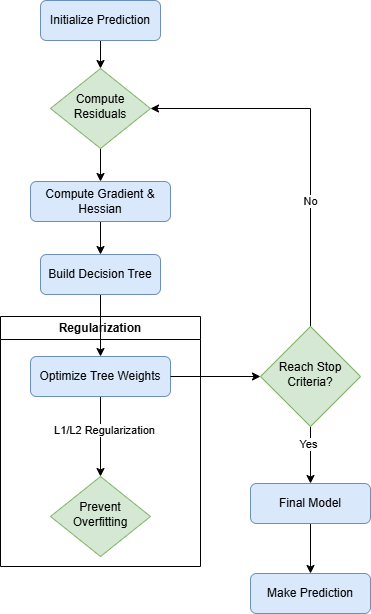
\includegraphics[width=0.5\textwidth]{XGBoost.png}
  \caption{Diagram of XGBooost algorithm.}
\end{figure}

\subsubsection{1.5 Make New Predictions}\label{make-new-predictions}

After training the model, for a test sample \(x\), XGBoost aggregates
the outputs of all trees: \[
\hat{y} = \sum_{k=1}^K f_k(x), \quad f_k \in \mathcal{F}
\] Where:

\begin{itemize}
\item
  \(f_k(x)\): The prediction from the \(k\)-th decision tree.
\item
  \(\mathcal{F}\): The set of all possible decision trees.
\end{itemize}

For classification problem, the output is often transformed into
probabilities using a sigmoid (binary) or softmax (multi-class)
function.

\subsubsection{1.6 Types of Problems Suitable for
XGBoost}\label{types-of-problems-suitable-for-xgboost}

XGBoost is suitable for solving regression on predicting continuous
values like stock price and classification problems like binary
classification and multi-class classification.

In Section C, I decide to solve a multi-class classification problem
using Car Evaluation (Bohanec 1988) data set provided by UC Irvine
machine learning repository.

\subsection{2. Introdction of Car Evaluation data
set}\label{introdction-of-car-evaluation-data-set}

Firstly, retrieving data using the UCI machine learning repository URL
and download it. However, the file only contains the data without the
columns' name. Therefore, I need to add the columns' name according to
the variables table (Bohanec 1988) , here is a screen shot of the
variables table:

\setcounter{figure}{1}
\begin{figure}
  \centering
  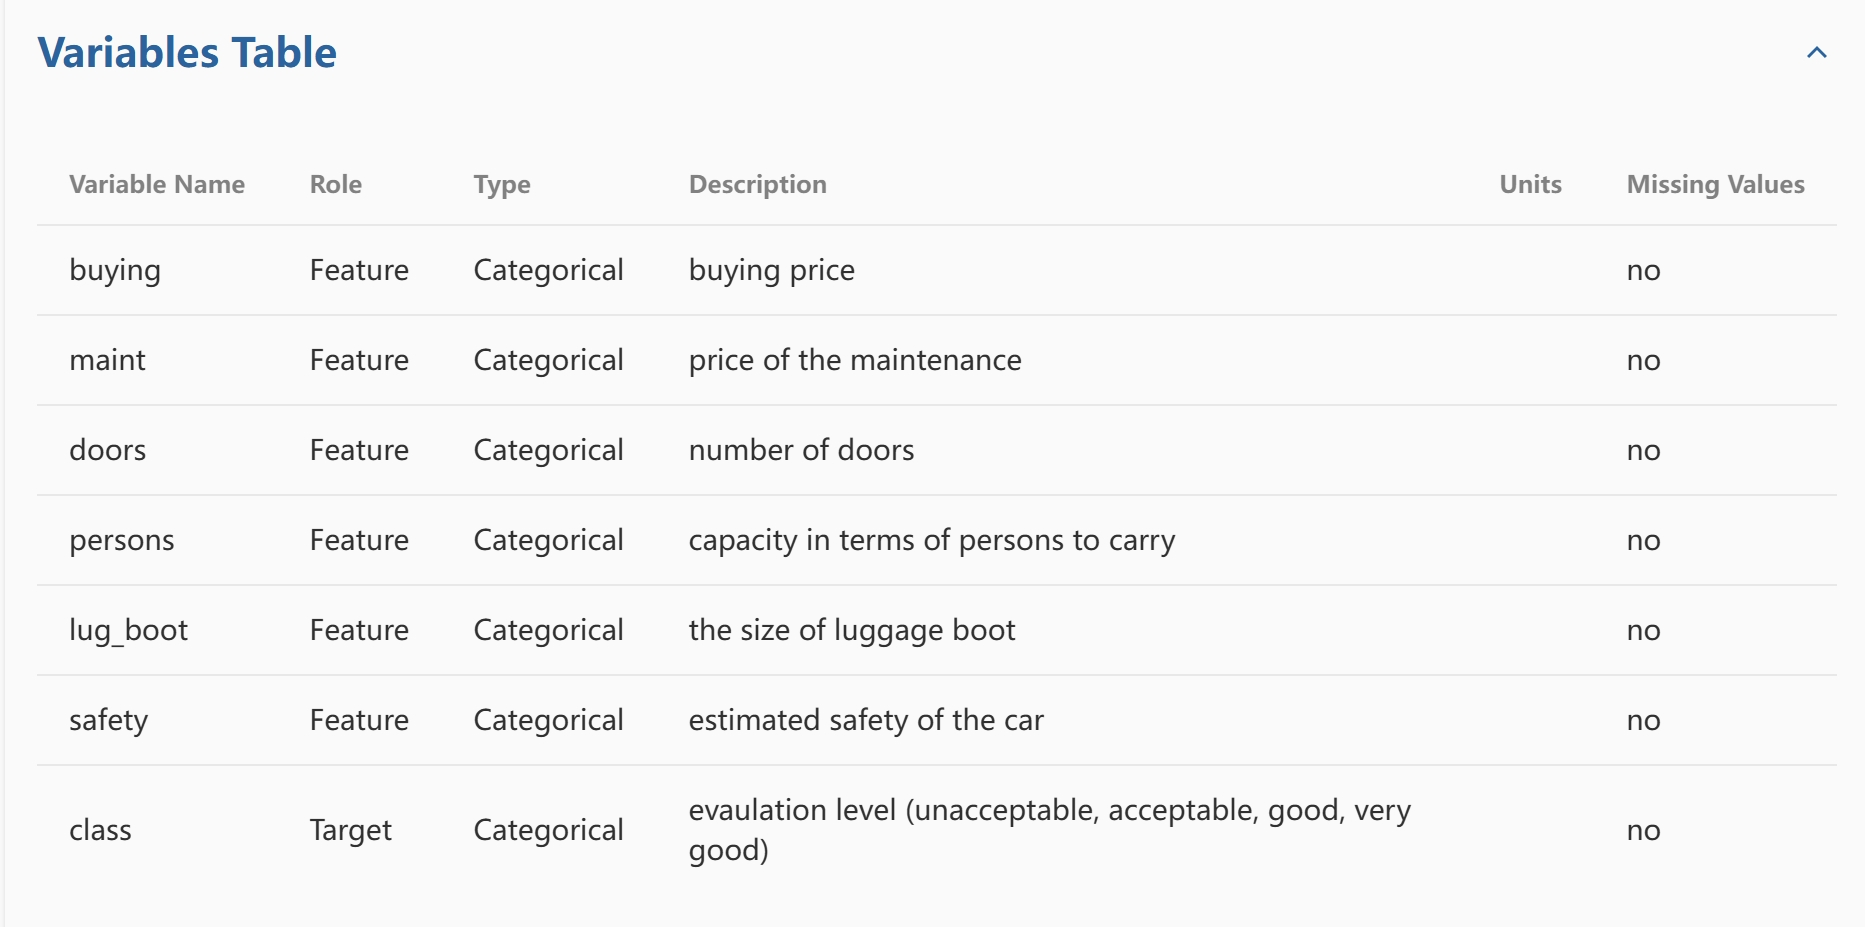
\includegraphics[width=0.8\textwidth]{VariablesTable.png}
  \caption{The variables table of Car Evaluation data set.}
\end{figure}

\begin{Shaded}
\begin{Highlighting}[]
\CommentTok{\# Download the Car Evaluation dataset}
\NormalTok{url }\OtherTok{=} \StringTok{"https://archive.ics.uci.edu/ml/machine{-}learning{-}databases/car/car.data"}
\NormalTok{data }\OtherTok{=} \FunctionTok{read.csv}\NormalTok{(url, }\AttributeTok{header =} \ConstantTok{FALSE}\NormalTok{, }\AttributeTok{stringsAsFactors =} \ConstantTok{TRUE}\NormalTok{)}

\CommentTok{\# Add column names}
\FunctionTok{colnames}\NormalTok{(data) }\OtherTok{\textless{}{-}} \FunctionTok{c}\NormalTok{(}\StringTok{"buying"}\NormalTok{, }\StringTok{"maint"}\NormalTok{, }\StringTok{"doors"}\NormalTok{, }\StringTok{"persons"}\NormalTok{, }\StringTok{"lug\_boot"}\NormalTok{, }\StringTok{"safety"}\NormalTok{, }\StringTok{"class"}\NormalTok{)}

\CommentTok{\# Check the structure of the data set}
\FunctionTok{str}\NormalTok{(data)}
\end{Highlighting}
\end{Shaded}

\begin{verbatim}
## 'data.frame':    1728 obs. of  7 variables:
##  $ buying  : Factor w/ 4 levels "high","low","med",..: 4 4 4 4 4 4 4 4 4 4 ...
##  $ maint   : Factor w/ 4 levels "high","low","med",..: 4 4 4 4 4 4 4 4 4 4 ...
##  $ doors   : Factor w/ 4 levels "2","3","4","5more": 1 1 1 1 1 1 1 1 1 1 ...
##  $ persons : Factor w/ 3 levels "2","4","more": 1 1 1 1 1 1 1 1 1 2 ...
##  $ lug_boot: Factor w/ 3 levels "big","med","small": 3 3 3 2 2 2 1 1 1 3 ...
##  $ safety  : Factor w/ 3 levels "high","low","med": 2 3 1 2 3 1 2 3 1 2 ...
##  $ class   : Factor w/ 4 levels "acc","good","unacc",..: 3 3 3 3 3 3 3 3 3 3 ...
\end{verbatim}

\begin{Shaded}
\begin{Highlighting}[]
\FunctionTok{table}\NormalTok{(data}\SpecialCharTok{$}\NormalTok{class)}
\end{Highlighting}
\end{Shaded}

\begin{verbatim}
## 
##   acc  good unacc vgood 
##   384    69  1210    65
\end{verbatim}

From Figure 2 and str() function, data set contains 1,728 examples and
six categorical features and one categorical target with no missing
values. Moreover, there are four classes in target value ``class'',
``unacc'' means unacceptable, ``acc'' mean acceptable, ``good'' means
the car is better than acceptable, and ``vgood'' means very good.
Therefore, multi-classification is well-suited for this data set.

However, by using table() function, most examples are concentrated in
one class, while the other classes have fewer instances. This imbalance
can lead to issues where the model performs well on the majority class
while poorly on the minority classes.

The goal of modeling Car Evaluation data set is using the supervised
learning method, which is XGBoost, to build a model to classify the cars
into four classes (unacceptable, acceptable, good and very good) based
on the six features. Since the data set only has 1,728 observations,
XGBoost is well-suited for this small data set, which means the accuracy
of the model would be higher.

In next part, I will apply XGBoost by R.

\subsection{3. Apply XGBoost}\label{apply-xgboost}

\subsubsection{3.1 Data Preprocessing}\label{data-preprocessing}

Firstly, load packages needed.

\begin{Shaded}
\begin{Highlighting}[]
\CommentTok{\# Load packages and do not show any messages}
\CommentTok{\# XGBoost package}
\FunctionTok{suppressMessages}\NormalTok{(}\FunctionTok{library}\NormalTok{(xgboost))}
\end{Highlighting}
\end{Shaded}

\begin{verbatim}
## Warning: 程序包'xgboost'是用R版本4.4.2 来建造的
\end{verbatim}

\begin{Shaded}
\begin{Highlighting}[]
\CommentTok{\# machine learning package}
\FunctionTok{suppressMessages}\NormalTok{(}\FunctionTok{library}\NormalTok{(caret))}
\end{Highlighting}
\end{Shaded}

\begin{verbatim}
## Warning: 程序包'caret'是用R版本4.4.2 来建造的
\end{verbatim}

\begin{Shaded}
\begin{Highlighting}[]
\CommentTok{\# data wrangling}
\FunctionTok{suppressMessages}\NormalTok{(}\FunctionTok{library}\NormalTok{(tidyverse))}

\CommentTok{\# data visualization}
\FunctionTok{suppressMessages}\NormalTok{(}\FunctionTok{library}\NormalTok{(ggplot2))}
\end{Highlighting}
\end{Shaded}

Then, preprocessing the raw data for later model training.

\begin{Shaded}
\begin{Highlighting}[]
\CommentTok{\# Convert the target variable \textquotesingle{}class\textquotesingle{} to numeric labels}
\CommentTok{\# XGBoost requires 0{-}based labels}
\NormalTok{data}\SpecialCharTok{$}\NormalTok{class }\OtherTok{=} \FunctionTok{as.numeric}\NormalTok{(}\FunctionTok{factor}\NormalTok{(data}\SpecialCharTok{$}\NormalTok{class)) }\SpecialCharTok{{-}} \DecValTok{1}
\end{Highlighting}
\end{Shaded}

Since XGBoost can not handle the raw categorical variables, I need to
transfer the categorical variables to dummy variables (dummy coding).

Dummy Coding is a method of representing categorical variables as binary
(0 or 1) variables in statistical models. It uses one category as the
reference level, and this reference category will not have its own
variable to avoid multicollinearity. If a dummy variable is created for
every category, this means that the sum of all dummy variables for a
single feature would always equal 1, leading to redundancy in the data.

\begin{Shaded}
\begin{Highlighting}[]
\CommentTok{\# Transform all raw categorical variables into dummy variables}
\CommentTok{\# Build full{-}rank dummy variables to avoid multicollinearity issues}
\NormalTok{dummies }\OtherTok{=} \FunctionTok{dummyVars}\NormalTok{(}\SpecialCharTok{\textasciitilde{}}\NormalTok{ ., }\AttributeTok{data =}\NormalTok{ data, }\AttributeTok{fullRank =} \ConstantTok{TRUE}\NormalTok{)}
\CommentTok{\# Build a new data frame that can be used for XGBoost}
\NormalTok{data\_transformed }\OtherTok{=} \FunctionTok{data.frame}\NormalTok{(}\FunctionTok{predict}\NormalTok{(dummies, }\AttributeTok{newdata =}\NormalTok{ data))}
\CommentTok{\# Check the structure of dummy variables}
\FunctionTok{str}\NormalTok{(data\_transformed)}
\end{Highlighting}
\end{Shaded}

\begin{verbatim}
## 'data.frame':    1728 obs. of  16 variables:
##  $ buying.low    : num  0 0 0 0 0 0 0 0 0 0 ...
##  $ buying.med    : num  0 0 0 0 0 0 0 0 0 0 ...
##  $ buying.vhigh  : num  1 1 1 1 1 1 1 1 1 1 ...
##  $ maint.low     : num  0 0 0 0 0 0 0 0 0 0 ...
##  $ maint.med     : num  0 0 0 0 0 0 0 0 0 0 ...
##  $ maint.vhigh   : num  1 1 1 1 1 1 1 1 1 1 ...
##  $ doors.3       : num  0 0 0 0 0 0 0 0 0 0 ...
##  $ doors.4       : num  0 0 0 0 0 0 0 0 0 0 ...
##  $ doors.5more   : num  0 0 0 0 0 0 0 0 0 0 ...
##  $ persons.4     : num  0 0 0 0 0 0 0 0 0 1 ...
##  $ persons.more  : num  0 0 0 0 0 0 0 0 0 0 ...
##  $ lug_boot.med  : num  0 0 0 1 1 1 0 0 0 0 ...
##  $ lug_boot.small: num  1 1 1 0 0 0 0 0 0 1 ...
##  $ safety.low    : num  1 0 0 1 0 0 1 0 0 1 ...
##  $ safety.med    : num  0 1 0 0 1 0 0 1 0 0 ...
##  $ class         : num  2 2 2 2 2 2 2 2 2 2 ...
\end{verbatim}

Next, I will set the hyper-parameters for the model. Hyper-parameters
are set before training, they control the model's learning process and
performance. Meanwhile, hyper-parameters are not learned from the data
but are instead set by the user and often tuned to optimize the model's
performance.

Here, I will set the hyper-parameters of XGBoost randomly, and later I
will try to use tuning techniques to find the best combination of
hyper-parameters.

\begin{Shaded}
\begin{Highlighting}[]
\CommentTok{\# Set hyper{-}parameters for the XGBoost model}
\NormalTok{params }\OtherTok{=} \FunctionTok{list}\NormalTok{(}
  \CommentTok{\# This is a multi{-}classification problem }
  \AttributeTok{objective =} \StringTok{"multi:softmax"}\NormalTok{,}
  \CommentTok{\# Number of classes}
  \AttributeTok{num\_class =} \FunctionTok{length}\NormalTok{(}\FunctionTok{unique}\NormalTok{(data\_transformed}\SpecialCharTok{$}\NormalTok{class)),  }
  \CommentTok{\# Learning rate}
  \AttributeTok{eta =} \FloatTok{0.1}\NormalTok{,}
  \CommentTok{\# Maximum depth of trees}
  \AttributeTok{max\_depth =} \DecValTok{6}\NormalTok{,}
  \CommentTok{\# Subsample ratio}
  \AttributeTok{subsample =} \FloatTok{0.8}\NormalTok{,}
  \CommentTok{\# Feature subsampling ratio}
  \AttributeTok{colsample\_bytree =} \FloatTok{0.8}\NormalTok{,}
  \CommentTok{\# Evaluation metric: classification error}
  \AttributeTok{eval\_metric =} \StringTok{"merror"}
\NormalTok{)}
\end{Highlighting}
\end{Shaded}

\subsubsection{3.2 Find Appropriate Performance
Metric}\label{find-appropriate-performance-metric}

Before starting model training, I still need to decide what performance
metric to use when evaluating the model.

As mentioned before, the data set is imbalanced, so using confusion
matrix and calculate the accuracy of this model is not appropriate
enough. The mathematical formula of accuracy is: \[
\text{Accuracy} = \frac{Number\,of\,Correct\,Prediction}{Total\,Prediction}
\] This metric only considers the proportion of correct predictions but
ignores the fact that there are more examples of ``unacc,'' which means
the model will perform better for this majority class. However, for the
minority class, such as ``vgood,'' the performance will not remain the
same. Therefore, the accuracy will looks higher when using this
imbalanced data set to train the model, but it can not represent the
true performance of the model.

However, the Weighted F1-Score can show the true performance of the
model better theoretically, because it evaluates precision and recall
for all classes, emphasizing correct classification of minority classes.

The formula of F1-Score for one class \(i\) is: \[
\text{F1-Score}_i = \frac{2 \cdot Precision_i \cdot Recall_i}{Precision_i + Recall_i}
\] Where: - Precision for class \(i\) is: \[
\text{Precision}_i = \frac{True Positives_i}{True Positives_i + False Positives_i}
\]

\begin{itemize}
\tightlist
\item
  Recall for class \(i\) is: \[
  \text{Recall}_i = \frac{True Positives_i}{True Positives_i + False Negatives_i}
  \] The Weighted F1-Score (Hinojosa Lee, Braet, and Springael 2024) is
  an improvement based on F1-Score, which adjusts the F1-Score for each
  class by adding a weight that is represented by the number of example
  in each class \(i\). \[
  \text{Weighted F1-Score} = \frac{\sum_{i=1}^C n_i \cdot \text{F1-Score}_i}{\sum_{i=1}^C n_i}
  \] Where:
\item
  \(C\) is the total number of classes.
\item
  \(n_i\) is the number of example in class \(i\).
\end{itemize}

According to the mathematical formula, I write a R function to calculate
Weighted F1-Score:

\begin{Shaded}
\begin{Highlighting}[]
\CommentTok{\# Function to calculate weighted F1{-}Score}
\NormalTok{weightedF1 }\OtherTok{=} \ControlFlowTok{function}\NormalTok{(true, pred) \{}
\NormalTok{  cm }\OtherTok{=} \FunctionTok{confusionMatrix}\NormalTok{(}\FunctionTok{as.factor}\NormalTok{(pred), }\FunctionTok{as.factor}\NormalTok{(true))}
  \CommentTok{\# Calculate precision according to confusion matrix}
\NormalTok{  precision }\OtherTok{=} \FunctionTok{diag}\NormalTok{(cm}\SpecialCharTok{$}\NormalTok{table) }\SpecialCharTok{/} \FunctionTok{rowSums}\NormalTok{(cm}\SpecialCharTok{$}\NormalTok{table)}
  
  \CommentTok{\# Calculate Recall according to confusion matrix}
\NormalTok{  recall }\OtherTok{=} \FunctionTok{diag}\NormalTok{(cm}\SpecialCharTok{$}\NormalTok{table) }\SpecialCharTok{/} \FunctionTok{colSums}\NormalTok{(cm}\SpecialCharTok{$}\NormalTok{table)}
  
  \CommentTok{\# Calculate F1{-}Score for each class}
\NormalTok{  f1 }\OtherTok{=} \DecValTok{2} \SpecialCharTok{*}\NormalTok{ (precision }\SpecialCharTok{*}\NormalTok{ recall) }\SpecialCharTok{/}\NormalTok{ (precision }\SpecialCharTok{+}\NormalTok{ recall)}
  
  \CommentTok{\# Combine the weight (Number of example in each class)}
\NormalTok{  weighted\_f1 }\OtherTok{=} \FunctionTok{sum}\NormalTok{(f1 }\SpecialCharTok{*} \FunctionTok{colSums}\NormalTok{(cm}\SpecialCharTok{$}\NormalTok{table) }\SpecialCharTok{/} \FunctionTok{sum}\NormalTok{(cm}\SpecialCharTok{$}\NormalTok{table), }\AttributeTok{na.rm =} \ConstantTok{TRUE}\NormalTok{)}
  \FunctionTok{return}\NormalTok{(weighted\_f1)}
\NormalTok{\}}
\end{Highlighting}
\end{Shaded}

Now, starting training process and calculate accuracy and Weighted
F1-Score then making comparison. Meanwhile, training data size will
varies and I will compare the performance of the model across different
sizes of training data. In the R code, the proportion of training set
starts from 0.2 to 0.9, increased by 0.05.

\begin{Shaded}
\begin{Highlighting}[]
\CommentTok{\# Initialize results storage}
\NormalTok{results }\OtherTok{=} \FunctionTok{data.frame}\NormalTok{(}\AttributeTok{T\_Size =} \FunctionTok{numeric}\NormalTok{(), }
                      \AttributeTok{T\_W\_F1 =} \FunctionTok{numeric}\NormalTok{(), }
                      \AttributeTok{Val\_W\_F1 =} \FunctionTok{numeric}\NormalTok{(),}
                      \AttributeTok{T\_Accuracy =} \FunctionTok{numeric}\NormalTok{(),}
                      \AttributeTok{Val\_Accuracy =} \FunctionTok{numeric}\NormalTok{())}

\CommentTok{\# Create a sequence to record different training size}
\NormalTok{training\_sizes }\OtherTok{=} \FunctionTok{seq}\NormalTok{(}\FloatTok{0.2}\NormalTok{, }\FloatTok{0.9}\NormalTok{, }\AttributeTok{by =} \FloatTok{0.05}\NormalTok{)}

\CommentTok{\# Train model using different training size}
\ControlFlowTok{for}\NormalTok{(size }\ControlFlowTok{in}\NormalTok{ training\_sizes)\{}
  \CommentTok{\# Create subset for training data}
\NormalTok{  subset\_index }\OtherTok{=} \FunctionTok{sample}\NormalTok{(}\DecValTok{1}\SpecialCharTok{:}\FunctionTok{nrow}\NormalTok{(data\_transformed), }\AttributeTok{size =} \FunctionTok{floor}\NormalTok{(size }\SpecialCharTok{*} \FunctionTok{nrow}\NormalTok{(data\_transformed)))}
\NormalTok{  subset\_train\_data }\OtherTok{=}\NormalTok{ data\_transformed[subset\_index, ]}
\NormalTok{  subset\_validation\_data }\OtherTok{=}\NormalTok{ data\_transformed[}\SpecialCharTok{{-}}\NormalTok{subset\_index, ]}

  \CommentTok{\# Separate features and target for training data}
\NormalTok{  X\_train\_subset }\OtherTok{=} \FunctionTok{as.matrix}\NormalTok{(subset\_train\_data[, }\SpecialCharTok{{-}}\FunctionTok{ncol}\NormalTok{(subset\_train\_data)])}
\NormalTok{  y\_train\_subset }\OtherTok{=}\NormalTok{ subset\_train\_data}\SpecialCharTok{$}\NormalTok{class}
  
  \CommentTok{\# Separate features and target for validation data}
\NormalTok{  X\_validation\_subset }\OtherTok{=} \FunctionTok{as.matrix}\NormalTok{(subset\_validation\_data[, }\SpecialCharTok{{-}}\FunctionTok{ncol}\NormalTok{(subset\_validation\_data)])}
\NormalTok{  y\_validation\_subset }\OtherTok{=}\NormalTok{ subset\_validation\_data}\SpecialCharTok{$}\NormalTok{class}
  
  \CommentTok{\# Convert data to DMatrix for XGBoost}
\NormalTok{  dtrain\_subset }\OtherTok{=} \FunctionTok{xgb.DMatrix}\NormalTok{(}\AttributeTok{data =}\NormalTok{ X\_train\_subset, }\AttributeTok{label =}\NormalTok{ y\_train\_subset)}
\NormalTok{  dvalidation\_subset }\OtherTok{=} \FunctionTok{xgb.DMatrix}\NormalTok{(}\AttributeTok{data =}\NormalTok{ X\_validation\_subset, }\AttributeTok{label =}\NormalTok{ y\_validation\_subset)}
  
  \CommentTok{\# Train XGBoost model}
\NormalTok{  model }\OtherTok{=} \FunctionTok{xgb.train}\NormalTok{(}\AttributeTok{params =}\NormalTok{ params, }
                     \AttributeTok{data =}\NormalTok{ dtrain\_subset, }
                     \AttributeTok{nrounds =} \DecValTok{50}\NormalTok{, }
                     \AttributeTok{watchlist =} \FunctionTok{list}\NormalTok{(}\AttributeTok{train =}\NormalTok{ dtrain\_subset, }\AttributeTok{val =}\NormalTok{ dvalidation\_subset),}
                     \AttributeTok{verbose =} \DecValTok{0}\NormalTok{)}
  
  \CommentTok{\# Predict on training data}
\NormalTok{  train\_preds }\OtherTok{=} \FunctionTok{predict}\NormalTok{(model, X\_train\_subset)}
  \CommentTok{\# Convert to class labels}
\NormalTok{  train\_preds }\OtherTok{=} \FunctionTok{as.integer}\NormalTok{(train\_preds) }
  
  \CommentTok{\# Predict on validation data}
\NormalTok{  validation\_preds }\OtherTok{=} \FunctionTok{predict}\NormalTok{(model, X\_validation\_subset)}
  \CommentTok{\# Convert to class labels}
\NormalTok{  validation\_preds }\OtherTok{=} \FunctionTok{as.integer}\NormalTok{(validation\_preds) }
  
  \CommentTok{\# Calculate Weighted F1{-}Scores}
\NormalTok{  train\_f1 }\OtherTok{=} \FunctionTok{weightedF1}\NormalTok{(y\_train\_subset, train\_preds)}
\NormalTok{  validation\_f1 }\OtherTok{=} \FunctionTok{weightedF1}\NormalTok{(y\_validation\_subset, validation\_preds)}
  
  \CommentTok{\# Calculate Accuracy}
\NormalTok{  train\_accuracy }\OtherTok{=} \FunctionTok{mean}\NormalTok{(train\_preds }\SpecialCharTok{==}\NormalTok{ y\_train\_subset)}
\NormalTok{  validation\_accuracy }\OtherTok{=} \FunctionTok{mean}\NormalTok{(validation\_preds }\SpecialCharTok{==}\NormalTok{ y\_validation\_subset)}
  
  \CommentTok{\# Store results}
\NormalTok{  results }\OtherTok{=} \FunctionTok{rbind}\NormalTok{(results, }\FunctionTok{data.frame}\NormalTok{(}\AttributeTok{T\_Size =}\NormalTok{ size, }
                                       \AttributeTok{T\_W\_F1 =}\NormalTok{ train\_f1, }
                                       \AttributeTok{Val\_W\_F1 =}\NormalTok{ validation\_f1,}
                                       \AttributeTok{T\_Accuracy =}\NormalTok{ train\_accuracy,}
                                       \AttributeTok{Val\_Accuracy =}\NormalTok{ validation\_accuracy))}
\NormalTok{\}}

\FunctionTok{print}\NormalTok{(results)}
\end{Highlighting}
\end{Shaded}

\begin{verbatim}
##    T_Size    T_W_F1  Val_W_F1 T_Accuracy Val_Accuracy
## 1    0.20 0.9913250 0.8867415  0.9913043    0.8893709
## 2    0.25 0.9839541 0.8922820  0.9837963    0.8927469
## 3    0.30 0.9922569 0.9035540  0.9922780    0.9041322
## 4    0.35 0.9884739 0.9015940  0.9884106    0.9056940
## 5    0.40 0.9913484 0.9106417  0.9913169    0.9112825
## 6    0.45 0.9819660 0.9057045  0.9819820    0.9095689
## 7    0.50 0.9814898 0.8760112  0.9814815    0.8912037
## 8    0.55 0.9864146 0.9222524  0.9863158    0.9280206
## 9    0.60 0.9827072 0.9092778  0.9826255    0.9118497
## 10   0.65 0.9806493 0.9269341  0.9804096    0.9272727
## 11   0.70 0.9777987 0.9495670  0.9776675    0.9499037
## 12   0.75 0.9786115 0.9363766  0.9783951    0.9375000
## 13   0.80 0.9784622 0.9584744  0.9782923    0.9595376
## 14   0.85 0.9816319 0.9048557  0.9816076    0.9076923
## 15   0.90 0.9802480 0.9400122  0.9800643    0.9421965
\end{verbatim}

From the result, both training Weighted F1-Score and training Accuracy
are very high (around 0.98), these show the XGBoost is a powerful
superivsed learning algorithm, and during training process, it can
achieve nearly perfect predictions for the training data.

However, the validation Accuracy and validation Weighted F1-Score are
not stable, varying dramatically from around 0.85 to around 0.93, and
they are much lower than the training metrics. This means that the model
performs well on the training data set but fails to generalize to
testing data, indicating that the model exists overfitting.

For a single columns, as the training data size grows, both the accuracy
and Weighted F1-Score will increase and the digits will reach the
highest point at around 0.8 to 1.0, which means it is suitable to set
around 80\% of the whole data set as training data.

Then I will create a plot for the result to help finding the trend.

\begin{Shaded}
\begin{Highlighting}[]
\CommentTok{\# Create a plot to show how F1{-}Score varies as the training data set increase}
\FunctionTok{ggplot}\NormalTok{(results, }\FunctionTok{aes}\NormalTok{(}\AttributeTok{x =}\NormalTok{ T\_Size)) }\SpecialCharTok{+}
  \FunctionTok{geom\_line}\NormalTok{(}\FunctionTok{aes}\NormalTok{(}\AttributeTok{y =}\NormalTok{ T\_W\_F1, }\AttributeTok{color =} \StringTok{"Training Weighted F1"}\NormalTok{)) }\SpecialCharTok{+}
  \FunctionTok{geom\_line}\NormalTok{(}\FunctionTok{aes}\NormalTok{(}\AttributeTok{y =}\NormalTok{ Val\_W\_F1, }\AttributeTok{color =} \StringTok{"Validation Weighted F1"}\NormalTok{)) }\SpecialCharTok{+}
  \FunctionTok{geom\_line}\NormalTok{(}\FunctionTok{aes}\NormalTok{(}\AttributeTok{y =}\NormalTok{ T\_Accuracy, }\AttributeTok{color =} \StringTok{"Training Accuracy"}\NormalTok{)) }\SpecialCharTok{+}
  \FunctionTok{geom\_line}\NormalTok{(}\FunctionTok{aes}\NormalTok{(}\AttributeTok{y =}\NormalTok{ Val\_Accuracy, }\AttributeTok{color =} \StringTok{"Validation Accuracy"}\NormalTok{)) }\SpecialCharTok{+}
  \FunctionTok{labs}\NormalTok{(}\AttributeTok{title =} \StringTok{"Figure 3: Performance Metrics vs Training Size"}\NormalTok{,}
       \AttributeTok{x =} \StringTok{"Training Data Size (Proportion)"}\NormalTok{, }
       \AttributeTok{y =} \StringTok{"Metrics"}\NormalTok{) }\SpecialCharTok{+}
  \FunctionTok{scale\_color\_manual}\NormalTok{(}\AttributeTok{name =} \StringTok{"Metrics"}\NormalTok{, }
                     \AttributeTok{values =} \FunctionTok{c}\NormalTok{(}\StringTok{"Training Weighted F1"} \OtherTok{=} \StringTok{"blue"}\NormalTok{, }
                                \StringTok{"Validation Weighted F1"} \OtherTok{=} \StringTok{"red"}\NormalTok{,}
                                \StringTok{"Training Accuracy"} \OtherTok{=} \StringTok{"green"}\NormalTok{,}
                                \StringTok{"Validation Accuracy"} \OtherTok{=} \StringTok{"orange"}\NormalTok{))  }\SpecialCharTok{+}
  \FunctionTok{theme\_minimal}\NormalTok{()}
\end{Highlighting}
\end{Shaded}

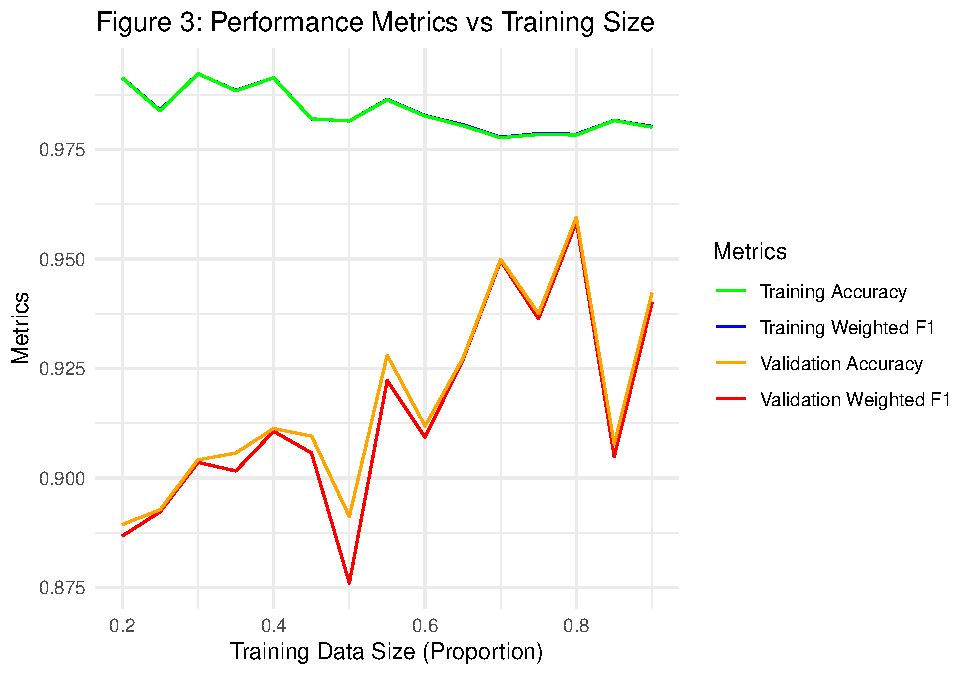
\includegraphics{Code_C_files/figure-latex/Create Plot-1.pdf}

From Figure 3, when training data size's proportion is lower than 0.7,
the gap between Training metrics and Validation metrics are very large,
which means too small training size leads to overfitting. When there is
not enough training data, the model will just memorize the results of
training data but can not make predictions on unseen data well, this can
lead to the large gap between Training and Validation metrics.

However, when the proportion of training data exceed 0.7, the Validation
metrics seems to reach the optimal region, which means the model
performance is optimal when training size is around 0.7 to 0.9.
Unfortunately, there still exists large gap between Training and
Validation metrics as the training size increases. To enhance the model
prediction performance, I will explore the impact of hyper-parameters
later.

Moreover, Training Accuracy and Training Weighted F1-Score are almost
the same (close to 1.0), maybe because the model performs high precision
and recalls for all classes on the training data. However, the
Validation Weighted F1-Score is slightly lower than the Validation
Accuracy when training data size is small, showing that the model is not
predicting minority classes well on new data. This is because Validation
Accuracy may overestimate performance because it doesn't penalize the
model for poor recall on minority classes as strongly as Weighted
F1-Score does.

Although the two metrics do not seem to have significant difference when
dealing with sufficient training sizes (over 0.7 proportion), Weighted
F1-Score still can be more reasonable for this imbalanced data set,
especially when dealing with small training sets. Therefore,
\textbf{Weighted F1-Score} is an appropriate metric for evaluating the
performance of XGBoost.

\subsubsection{3.3 Impact of Different Training Set
Sizes}\label{impact-of-different-training-set-sizes}

Next, I will explain the impact of different training data size. From
Figure 3, I observe that the Training Weighted F1-Score remains high
(close to 1) across all training size. This suggests that the XGBoost
performs well on training data, even with small training data sizes.

However, Validation Weighted F1-Score starts lower for smaller training
sizes and increases as the training size grows, which means the
insufficient training size has negative impact on the model's
generalization. As training size increases, the gap between training and
validation performance decreases, meaning the model performs better with
larger training size.

Additionally, at around 70\% to 90\% training size, the Validation
Weighted F1-Score converges and reaches a satisfactory level. Therefore,
a training size of approximately 80\% seems to provide the optimal
balance between performance and efficiency, as adding more data beyond
this point provides minimal improvement or even negative impact.
Therefore, in later model adjustment, I will keep using 80\% of the
whole data set as the training size.

\subsection{\texorpdfstring{4. Impact on varying learning rate
\(\eta\)}{4. Impact on varying learning rate \textbackslash eta}}\label{impact-on-varying-learning-rate-eta}

This part will explore how the performance of XGBoost model varies on
both the training data and the validation data as as the learning rate
\(\eta\) (a hyper-parameter) is varied.

Learning rate, as a hyper-parameter, its value is between 0 to 1 and it
determines the step size during optimization. Smaller values lead to
better generalization but may require more boosting rounds, increasing
cost of computation. In contrast, larger values make the process faster,
but potentially increase the risk of overfitting.

Firstly, I will train the model with different learning rate and record
the Weighted F1-Score.

\begin{Shaded}
\begin{Highlighting}[]
\CommentTok{\# Learning rate sequence}
\NormalTok{learning\_rates }\OtherTok{=} \FunctionTok{seq}\NormalTok{(}\FloatTok{0.01}\NormalTok{, }\DecValTok{1}\NormalTok{, }\AttributeTok{by=}\FloatTok{0.05}\NormalTok{)}

\CommentTok{\# Create result for different learning rate}
\NormalTok{results\_rl }\OtherTok{=} \FunctionTok{data.frame}\NormalTok{(}\AttributeTok{learning\_rate =} \FunctionTok{numeric}\NormalTok{(), }
                     \AttributeTok{T\_W\_F1 =} \FunctionTok{numeric}\NormalTok{(), }
                     \AttributeTok{Val\_W\_F1 =} \FunctionTok{numeric}\NormalTok{())}

\CommentTok{\# Set params without learning rate, adjust learning rate in each iteration}
\NormalTok{params }\OtherTok{=} \FunctionTok{list}\NormalTok{(}
        \AttributeTok{objective =} \StringTok{"multi:softmax"}\NormalTok{,}
        \AttributeTok{num\_class =} \FunctionTok{length}\NormalTok{(}\FunctionTok{unique}\NormalTok{(data\_transformed}\SpecialCharTok{$}\NormalTok{class)),}
        \AttributeTok{eval\_metric =} \StringTok{"merror"}\NormalTok{,}
        \AttributeTok{max\_depth =} \DecValTok{6}\NormalTok{,}
        \AttributeTok{subsample =} \FloatTok{0.8}\NormalTok{,}
        \AttributeTok{colsample\_bytree =} \FloatTok{0.8}
\NormalTok{    )}

\CommentTok{\# Set 80\% training and 20\% validation data}
\NormalTok{train\_index }\OtherTok{=} \FunctionTok{createDataPartition}\NormalTok{(data\_transformed}\SpecialCharTok{$}\NormalTok{class, }\AttributeTok{p =} \FloatTok{0.8}\NormalTok{, }\AttributeTok{list =} \ConstantTok{FALSE}\NormalTok{)}
\NormalTok{train\_data }\OtherTok{=}\NormalTok{ data\_transformed[train\_index, ]}
\NormalTok{validation\_data }\OtherTok{=}\NormalTok{ data\_transformed[}\SpecialCharTok{{-}}\NormalTok{train\_index, ]}

\CommentTok{\# Separate features and target for training and validation data}
\NormalTok{X\_train }\OtherTok{=} \FunctionTok{as.matrix}\NormalTok{(train\_data[, }\SpecialCharTok{{-}}\FunctionTok{ncol}\NormalTok{(train\_data)])}
\NormalTok{y\_train }\OtherTok{=}\NormalTok{ train\_data}\SpecialCharTok{$}\NormalTok{class}
\NormalTok{X\_validation }\OtherTok{=} \FunctionTok{as.matrix}\NormalTok{(validation\_data[, }\SpecialCharTok{{-}}\FunctionTok{ncol}\NormalTok{(validation\_data)])}
\NormalTok{y\_validation }\OtherTok{=}\NormalTok{ validation\_data}\SpecialCharTok{$}\NormalTok{class}

\CommentTok{\# Convert training and validation data to DMatrix format for XGBoost}
\NormalTok{dtrain }\OtherTok{=} \FunctionTok{xgb.DMatrix}\NormalTok{(}\AttributeTok{data =}\NormalTok{ X\_train, }\AttributeTok{label =}\NormalTok{ y\_train)}
\NormalTok{dvalidation }\OtherTok{=} \FunctionTok{xgb.DMatrix}\NormalTok{(}\AttributeTok{data =}\NormalTok{ X\_validation, }\AttributeTok{label =}\NormalTok{ y\_validation)}

\ControlFlowTok{for}\NormalTok{ (lr }\ControlFlowTok{in}\NormalTok{ learning\_rates) \{}
  
  \CommentTok{\# Update the learning rate in the parameters}
\NormalTok{  params}\SpecialCharTok{$}\NormalTok{eta }\OtherTok{=}\NormalTok{ lr}

  \CommentTok{\# Train the XGBoost model}
\NormalTok{  model }\OtherTok{\textless{}{-}} \FunctionTok{xgb.train}\NormalTok{(}\AttributeTok{params =}\NormalTok{ params, }
                     \AttributeTok{data =}\NormalTok{ dtrain, }
                     \AttributeTok{nrounds =} \DecValTok{50}\NormalTok{, }
                     \AttributeTok{watchlist =} \FunctionTok{list}\NormalTok{(}\AttributeTok{train =}\NormalTok{ dtrain, }\AttributeTok{val =}\NormalTok{ dvalidation),}
                     \AttributeTok{verbose =} \DecValTok{0}\NormalTok{)}
  
  \CommentTok{\# Predictions on training and validation data}
\NormalTok{  train\_preds }\OtherTok{=} \FunctionTok{predict}\NormalTok{(model, X\_train)}
\NormalTok{  train\_preds }\OtherTok{=} \FunctionTok{as.integer}\NormalTok{(train\_preds)}
\NormalTok{  validation\_preds }\OtherTok{=} \FunctionTok{predict}\NormalTok{(model, X\_validation)}
\NormalTok{  validation\_preds }\OtherTok{=} \FunctionTok{as.integer}\NormalTok{(validation\_preds)}
  
  \CommentTok{\# Calculate Weighted F1{-}Score for both training and validation sets}
\NormalTok{  train\_f1 }\OtherTok{=} \FunctionTok{weightedF1}\NormalTok{(y\_train, train\_preds)}
\NormalTok{  validation\_f1 }\OtherTok{=} \FunctionTok{weightedF1}\NormalTok{(y\_validation, validation\_preds)}
  
  \CommentTok{\# Store the results}
\NormalTok{  results\_rl }\OtherTok{=} \FunctionTok{rbind}\NormalTok{(results\_rl, }\FunctionTok{data.frame}\NormalTok{(}\AttributeTok{learning\_rate =}\NormalTok{ lr, }
                                       \AttributeTok{train\_W\_F1 =}\NormalTok{ train\_f1, }
                                       \AttributeTok{Val\_W\_F1 =}\NormalTok{ validation\_f1))}
\NormalTok{\}}
\FunctionTok{head}\NormalTok{(results\_rl)}
\end{Highlighting}
\end{Shaded}

\begin{verbatim}
##   learning_rate train_W_F1  Val_W_F1
## 1          0.01  0.9269328 0.8622449
## 2          0.06  0.9592251 0.8954863
## 3          0.11  0.9813359 0.9420609
## 4          0.16  0.9949666 0.9682253
## 5          0.21  0.9971192 0.9714195
## 6          0.26  1.0000000 0.9740279
\end{verbatim}

\begin{Shaded}
\begin{Highlighting}[]
\CommentTok{\# Plot the results}
\FunctionTok{ggplot}\NormalTok{(results\_rl, }\FunctionTok{aes}\NormalTok{(}\AttributeTok{x =}\NormalTok{ learning\_rate)) }\SpecialCharTok{+}
  \FunctionTok{geom\_smooth}\NormalTok{(}\FunctionTok{aes}\NormalTok{(}\AttributeTok{y =}\NormalTok{ train\_W\_F1, }\AttributeTok{color =} \StringTok{"Training Weighted F1{-}Score"}\NormalTok{)) }\SpecialCharTok{+}
  \FunctionTok{geom\_smooth}\NormalTok{(}\FunctionTok{aes}\NormalTok{(}\AttributeTok{y =}\NormalTok{ Val\_W\_F1, }\AttributeTok{color =} \StringTok{"Validation Weighted F1{-}Score"}\NormalTok{)) }\SpecialCharTok{+}
  \FunctionTok{scale\_color\_manual}\NormalTok{(}\AttributeTok{values =} \FunctionTok{c}\NormalTok{(}\StringTok{"Training Weighted F1{-}Score"} \OtherTok{=} \StringTok{"cyan"}\NormalTok{,}
                                \StringTok{"Validation Weighted F1{-}Score"} \OtherTok{=} \StringTok{"brown"}\NormalTok{)) }\SpecialCharTok{+}
  \FunctionTok{labs}\NormalTok{(}\AttributeTok{title =} \StringTok{"Figure 4 Weighted F1{-}Score vs Learning Rate"}\NormalTok{,}
       \AttributeTok{x =} \StringTok{"Learning Rate"}\NormalTok{, }\AttributeTok{y =} \StringTok{"Weighted F1{-}Score"}\NormalTok{) }\SpecialCharTok{+}
  \FunctionTok{theme\_minimal}\NormalTok{()}
\end{Highlighting}
\end{Shaded}

\begin{verbatim}
## `geom_smooth()` using method = 'loess' and formula = 'y ~ x'
## `geom_smooth()` using method = 'loess' and formula = 'y ~ x'
\end{verbatim}

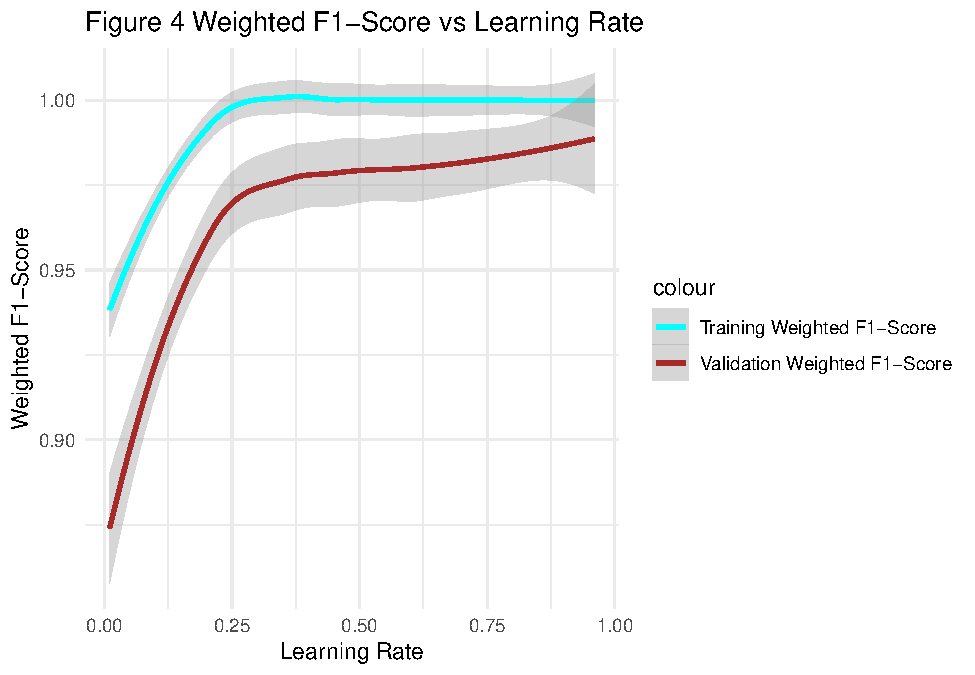
\includegraphics{Code_C_files/figure-latex/plot for different learning rate-1.pdf}
From Figure 4, it is obvious that the Validation Weighted F1-Score
increases sharply (from around 0.93 to around 0.97) as the learning rate
increase from 0.01 to 0.25. However, when the learning rate exceeds
0.25, both the training and validation Weighted F1-Scores' curves
converge to nearly a straight line. These observations indicate that the
best learning rate for this model is around 0.25. Moreover, if using a
larger learning rate than 0.25, it will lead to a higher risk of
overfitting.

\subsection{5 Find optiaml learning rate using
cross-validation}\label{find-optiaml-learning-rate-using-cross-validation}

\subsubsection{5.1 Introduce
Cross-validation}\label{introduce-cross-validation}

To validate the observation from Figure 4, cross-validation will be used
to accurately determine the optimal learning rate for this model (Arlot
and Celisse 2010).

Cross-validation (CV) splits data set into several training and
validation folds to help evaluate model performance. It reduces the risk
of overfitting or underfitting compared to a single train-validation
split. Moreover, CV is useful to help finding optimal hyper-parameters
before training the final model.

Here is a diagram of 5-fold cross-validation:

\setcounter{figure}{4}
\begin{figure}
  \centering
  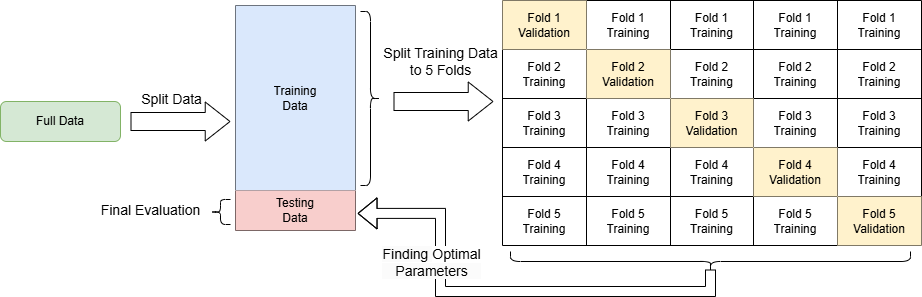
\includegraphics[width=0.8\textwidth]{Cross_validation.png}
  \caption{The diagram of 5-fold cross-validation.}
\end{figure}

Now apply CV to find the optimal learning rate.

\begin{Shaded}
\begin{Highlighting}[]
\CommentTok{\# Based on Figure 4, we just need to validate several typical learning rate}
\NormalTok{learning\_rates }\OtherTok{=} \FunctionTok{seq}\NormalTok{(}\FloatTok{0.1}\NormalTok{, }\FloatTok{0.3}\NormalTok{, }\AttributeTok{by =} \FloatTok{0.01}\NormalTok{)}

\CommentTok{\# Storage for cross{-}validation results}
\NormalTok{cv\_results }\OtherTok{=} \FunctionTok{data.frame}\NormalTok{(}\AttributeTok{learning\_rate =} \FunctionTok{numeric}\NormalTok{(), }
                         \AttributeTok{train\_merror\_mean =} \FunctionTok{numeric}\NormalTok{(), }
                         \AttributeTok{test\_merror\_mean =} \FunctionTok{numeric}\NormalTok{())}

\NormalTok{params }\OtherTok{=} \FunctionTok{list}\NormalTok{(}
  \AttributeTok{objective =} \StringTok{"multi:softmax"}\NormalTok{,}
  \AttributeTok{num\_class =} \FunctionTok{length}\NormalTok{(}\FunctionTok{unique}\NormalTok{(data\_transformed}\SpecialCharTok{$}\NormalTok{class)),}
  \AttributeTok{eta =}\NormalTok{ lr,}
  \AttributeTok{max\_depth =} \DecValTok{6}\NormalTok{,}
  \AttributeTok{subsample =} \FloatTok{0.8}\NormalTok{,}
  \AttributeTok{colsample\_bytree =} \FloatTok{0.8}\NormalTok{,}
  \AttributeTok{eval\_metric =} \StringTok{"merror"}
\NormalTok{)}
\CommentTok{\# Perform Cross{-}Validation for Each Learning Rate}
\FunctionTok{set.seed}\NormalTok{(}\DecValTok{333}\NormalTok{)}
\ControlFlowTok{for}\NormalTok{ (lr }\ControlFlowTok{in}\NormalTok{ learning\_rates) \{}
  \CommentTok{\# Update the learning rate in parameters}
\NormalTok{  params}\SpecialCharTok{$}\NormalTok{eta }\OtherTok{=}\NormalTok{ lr}
  
  \CommentTok{\# Try 5{-}Fold Cross{-}Validation}
\NormalTok{  cv }\OtherTok{=} \FunctionTok{xgb.cv}\NormalTok{(}
    \AttributeTok{params =}\NormalTok{ params,}
    \AttributeTok{data =}\NormalTok{ dtrain,}
    \AttributeTok{nfold =} \DecValTok{5}\NormalTok{,}
    \AttributeTok{nrounds =} \DecValTok{50}\NormalTok{,}
    \AttributeTok{verbose =} \DecValTok{0}\NormalTok{,}
    \AttributeTok{stratified =} \ConstantTok{TRUE}
\NormalTok{  )}
  
  \CommentTok{\# Store Average Train and Validation F1{-}Score}
\NormalTok{  train\_merror\_mean }\OtherTok{=} \FunctionTok{mean}\NormalTok{(cv}\SpecialCharTok{$}\NormalTok{evaluation\_log}\SpecialCharTok{$}\NormalTok{train\_merror\_mean)}
\NormalTok{  test\_merror\_mean }\OtherTok{=} \FunctionTok{mean}\NormalTok{(cv}\SpecialCharTok{$}\NormalTok{evaluation\_log}\SpecialCharTok{$}\NormalTok{test\_merror\_mean)}
  
\NormalTok{  cv\_results }\OtherTok{=} \FunctionTok{rbind}\NormalTok{(cv\_results, }\FunctionTok{data.frame}\NormalTok{(}\AttributeTok{learning\_rate =}\NormalTok{ lr, }
                                             \AttributeTok{train\_merror\_mean =}\NormalTok{ train\_merror\_mean, }
                                             \AttributeTok{test\_merror\_mean =}\NormalTok{ test\_merror\_mean))}
\NormalTok{\}}

\FunctionTok{ggplot}\NormalTok{(cv\_results, }\FunctionTok{aes}\NormalTok{(}\AttributeTok{x =}\NormalTok{ learning\_rate)) }\SpecialCharTok{+}
  \FunctionTok{geom\_smooth}\NormalTok{(}\FunctionTok{aes}\NormalTok{(}\AttributeTok{y =}\NormalTok{ train\_merror\_mean, }\AttributeTok{color =} \StringTok{"Training merror mean"}\NormalTok{)) }\SpecialCharTok{+}
  \FunctionTok{geom\_smooth}\NormalTok{(}\FunctionTok{aes}\NormalTok{(}\AttributeTok{y =}\NormalTok{ test\_merror\_mean, }\AttributeTok{color =} \StringTok{"Test merror mean"}\NormalTok{)) }\SpecialCharTok{+}
  \FunctionTok{scale\_color\_manual}\NormalTok{(}\AttributeTok{values =} \FunctionTok{c}\NormalTok{(}\StringTok{"Training merror mean"} \OtherTok{=} \StringTok{"blue"}\NormalTok{,}
                                \StringTok{"Test merror mean"} \OtherTok{=} \StringTok{"red"}\NormalTok{)) }\SpecialCharTok{+}
  \FunctionTok{labs}\NormalTok{(}\AttributeTok{title =} \StringTok{"Figure 6 merror mean vs Learning Rate by cross{-}validation"}\NormalTok{,}
       \AttributeTok{x =} \StringTok{"Learning Rate"}\NormalTok{, }\AttributeTok{y =} \StringTok{"merror mean"}\NormalTok{) }\SpecialCharTok{+}
  \FunctionTok{theme\_minimal}\NormalTok{()}
\end{Highlighting}
\end{Shaded}

\begin{verbatim}
## `geom_smooth()` using method = 'loess' and formula = 'y ~ x'
## `geom_smooth()` using method = 'loess' and formula = 'y ~ x'
\end{verbatim}

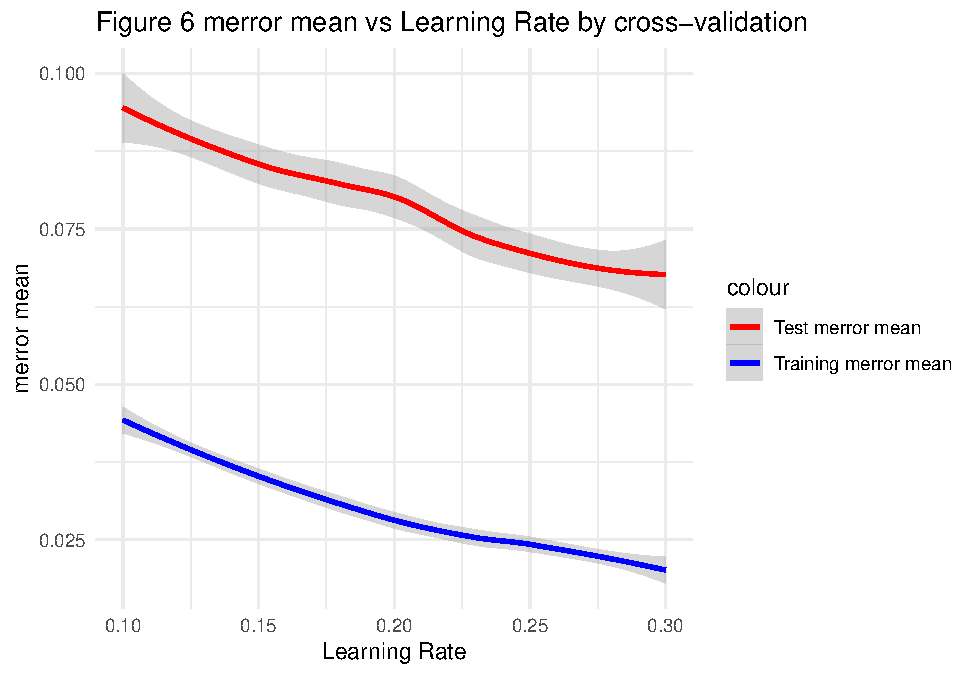
\includegraphics{Code_C_files/figure-latex/cross-validation to find optimal learning rate-1.pdf}
From Figure 6, it is evident that the merror mean decreases sharply as
the learning rate increases from 0.1 to around 0.25. After that, the
decrease slows down, which indicates that the best learning rate should
be around 0.25 to 0.3.

However, the graph is still not direct for choosing the best learning
rate, because the optimal learning rate should ensure that the test
error is low while keeping the training error relatively close.
Therefore, I can search the minimal test\_merror\_mean in results and
this point's learning rate can be considered as best learning rate. This
test\_merror\_mean is the average misclassification error across all
cross-validation folds, and misclassification error is a metric
represents the proportion of incorrectly classified instances out of the
total instances.

The formula of merror\_mean is:

\[
\text{Mislcassification_Error_Mean}=\frac{1}{K} \sum_{k=1}^{K} \frac{1}{N_k}\sum_{i=1}^{N_k}\frac{Number\ of\ Incorrect\ Predictions}{Total\ Predictions}
\]

Where: - \(K\): The total number of folds or iterations in the
cross-validation process. - \(N_k\): The number of instances (samples)
in the \(k\)-th fold.

When merror\_mean reach its minimal, this means the model's performance
is optimal at this learning rate.

\begin{Shaded}
\begin{Highlighting}[]
\CommentTok{\# Find the minimal test merror mean, this point can be the best learning rate}
\NormalTok{best\_lr }\OtherTok{=}\NormalTok{ cv\_results[}\FunctionTok{which.min}\NormalTok{(cv\_results}\SpecialCharTok{$}\NormalTok{test\_merror\_mean), }\StringTok{"learning\_rate"}\NormalTok{]}
\FunctionTok{print}\NormalTok{(}\FunctionTok{paste}\NormalTok{(}\StringTok{"Best Learning Rate:"}\NormalTok{, best\_lr))}
\end{Highlighting}
\end{Shaded}

\begin{verbatim}
## [1] "Best Learning Rate: 0.29"
\end{verbatim}

\subsubsection{5.2 Fit New Model}\label{fit-new-model}

Then we can apply the best learning rate to build the adjusted model and
create a test data to evaluate the performance of it.

\begin{Shaded}
\begin{Highlighting}[]
\CommentTok{\# Train Final Model with Best Learning Rate}
\NormalTok{params}\SpecialCharTok{$}\NormalTok{eta }\OtherTok{=}\NormalTok{ best\_lr}
\NormalTok{adjusted\_model }\OtherTok{=} \FunctionTok{xgb.train}\NormalTok{(}
  \AttributeTok{params =}\NormalTok{ params,}
  \AttributeTok{data =}\NormalTok{ dtrain,}
  \AttributeTok{nrounds =} \DecValTok{50}
\NormalTok{)}
\NormalTok{test\_data }\OtherTok{=}\NormalTok{ data\_transformed[}\SpecialCharTok{{-}}\NormalTok{train\_index,]}
\CommentTok{\# Predict on Test Data}
\NormalTok{test\_preds }\OtherTok{=} \FunctionTok{predict}\NormalTok{(adjusted\_model, }\FunctionTok{as.matrix}\NormalTok{(test\_data[, }\SpecialCharTok{{-}}\FunctionTok{ncol}\NormalTok{(test\_data)]))}
\NormalTok{test\_preds }\OtherTok{=} \FunctionTok{as.integer}\NormalTok{(test\_preds)}

\CommentTok{\# Calculate Weighted F1{-}Score on Test Data}
\NormalTok{test\_f1 }\OtherTok{=} \FunctionTok{weightedF1}\NormalTok{(test\_data}\SpecialCharTok{$}\NormalTok{class, test\_preds)}

\NormalTok{original\_f1 }\OtherTok{=}\NormalTok{ results[}\DecValTok{7}\NormalTok{,]}\SpecialCharTok{$}\NormalTok{Val\_W\_F1}
\FunctionTok{cat}\NormalTok{(}\StringTok{"Test Weighted F1{-}Score of Adjusted Model:"}\NormalTok{, test\_f1,}\StringTok{"}\SpecialCharTok{\textbackslash{}n}\StringTok{"}\NormalTok{)}
\end{Highlighting}
\end{Shaded}

\begin{verbatim}
## Test Weighted F1-Score of Adjusted Model: 0.9738149
\end{verbatim}

\begin{Shaded}
\begin{Highlighting}[]
\FunctionTok{cat}\NormalTok{(}\StringTok{"Test Weighted F1{-}Score of Original Model:"}\NormalTok{, original\_f1, }\StringTok{"}\SpecialCharTok{\textbackslash{}n}\StringTok{"}\NormalTok{)}
\end{Highlighting}
\end{Shaded}

\begin{verbatim}
## Test Weighted F1-Score of Original Model: 0.8760112
\end{verbatim}

From the comparison of the Test Weighted F1-Score between the adjusted
model and the original model, it is obvious that the Weighted F1-Score
of adjusted model is larger than that of the original model, indicating
the cross-validation is useful for finding the optimal hyper-parameters
for fitting a better model.

Therefore, cross-validation is still a useful method to guide the search
for optimal hyper-parameters and to fit a more well-performing model.

\subsection{6 Grid Search to find optimal
hyper-parameters}\label{grid-search-to-find-optimal-hyper-parameters}

\subsubsection{6.1 Introduce Grid Search}\label{introduce-grid-search}

After finding an optimal learning rate, the adjusted model's Weighted
F1-Score is much higher than the origianl model. However, I did not
consider the correlation between hyper-parameters, and this ``optimal''
learning rate may not be optimal when changing other hyper-parameters.
Therefore, to enhance the model further, I need to find a set of
hyper-parameters that can make the model perform better than previous.
In this part, I will use Grid Search.

Grid Search is a method used for hyper-parameter optimization in machine
learning. (Bergstra et al. 2011) It uses exhaustively searching through
a predefined set of hyper-parameters to find a combination that produces
the best performance for a model.

To apply grid search, firstly, I need to select a set of
hyper-parameters of the model I want to tune, and for each
hyper-parameter, I need to provide a list of possible values. Then,
generating all possible combinations of the hyperparameter values as a
grid. The last step is training and evaluating the model using
cross-validation to find the best combination.

\begin{Shaded}
\begin{Highlighting}[]
\CommentTok{\# Grid search for hyper{-}parameter tuning}

\CommentTok{\# Prepare possible hyper{-}parameters sequence for grid search}
\NormalTok{tune\_grid }\OtherTok{=} \FunctionTok{expand.grid}\NormalTok{(}
  \CommentTok{\# The number of boosting rounds}
  \AttributeTok{nrounds =} \FunctionTok{c}\NormalTok{(}\DecValTok{50}\NormalTok{, }\DecValTok{100}\NormalTok{, }\DecValTok{150}\NormalTok{),}
  
  \CommentTok{\# The maximum depth of each decision tree}
  \AttributeTok{max\_depth =} \FunctionTok{c}\NormalTok{(}\DecValTok{4}\NormalTok{, }\DecValTok{6}\NormalTok{, }\DecValTok{8}\NormalTok{),}
  
  \CommentTok{\# The learning rate}
  \AttributeTok{eta =} \FunctionTok{c}\NormalTok{(}\FloatTok{0.01}\NormalTok{, }\FloatTok{0.1}\NormalTok{, best\_lr),}
  
  \CommentTok{\# Regularization term}
  \AttributeTok{gamma =} \FunctionTok{c}\NormalTok{(}\DecValTok{0}\NormalTok{, }\FloatTok{0.1}\NormalTok{, }\FloatTok{0.2}\NormalTok{),}
  
  \CommentTok{\# The fraction of features to sample randomly for each tree.}
  \AttributeTok{colsample\_bytree =} \FunctionTok{c}\NormalTok{(}\FloatTok{0.8}\NormalTok{, }\FloatTok{1.0}\NormalTok{),}
  
  \CommentTok{\# The minimum sum of instance weights (hessian) required in a child node}
  \AttributeTok{min\_child\_weight =} \FunctionTok{c}\NormalTok{(}\DecValTok{1}\NormalTok{, }\DecValTok{3}\NormalTok{),}
  
  \CommentTok{\# The fraction of training data to sample randomly for building each tree.}
  \AttributeTok{subsample =} \FunctionTok{c}\NormalTok{(}\FloatTok{0.8}\NormalTok{, }\FloatTok{1.0}\NormalTok{)}
\NormalTok{)}

\CommentTok{\# Function to evaluate a set of parameters}
\NormalTok{eval\_params }\OtherTok{=} \ControlFlowTok{function}\NormalTok{(nrounds, max\_depth, eta, gamma, }
\NormalTok{                       colsample\_bytree, min\_child\_weight, subsample) \{}
  \CommentTok{\# Set hyper{-}parameters}
\NormalTok{  params }\OtherTok{=} \FunctionTok{list}\NormalTok{(}
    \AttributeTok{objective =} \StringTok{"multi:softmax"}\NormalTok{,}
    \AttributeTok{num\_class =} \FunctionTok{length}\NormalTok{(}\FunctionTok{unique}\NormalTok{(data\_transformed}\SpecialCharTok{$}\NormalTok{class)),}
    \AttributeTok{max\_depth =}\NormalTok{ max\_depth,}
    \AttributeTok{eta =}\NormalTok{ eta,}
    \AttributeTok{gamma =}\NormalTok{ gamma,}
    \AttributeTok{colsample\_bytree =}\NormalTok{ colsample\_bytree,}
    \AttributeTok{min\_child\_weight =}\NormalTok{ min\_child\_weight,}
    \AttributeTok{subsample =}\NormalTok{ subsample}
\NormalTok{  )}
  
  \CommentTok{\# Use cross{-}validation to find the optimal\_params }
\NormalTok{  cv }\OtherTok{=} \FunctionTok{xgb.cv}\NormalTok{(}
    \AttributeTok{params =}\NormalTok{ params,}
    \AttributeTok{data =}\NormalTok{ dtrain,}
    \AttributeTok{nrounds =}\NormalTok{ nrounds,}
    \AttributeTok{nfold =} \DecValTok{5}\NormalTok{,}
    \AttributeTok{early\_stopping\_rounds =} \DecValTok{10}\NormalTok{,}
    \AttributeTok{metrics =} \StringTok{"merror"}\NormalTok{,}
    \AttributeTok{verbose =} \ConstantTok{FALSE}
\NormalTok{  )}
  
  \FunctionTok{return}\NormalTok{(}\FunctionTok{min}\NormalTok{(cv}\SpecialCharTok{$}\NormalTok{evaluation\_log}\SpecialCharTok{$}\NormalTok{test\_merror\_mean))}
\NormalTok{\}}

\CommentTok{\# Perform grid search}
\NormalTok{results\_gs }\OtherTok{=} \FunctionTok{apply}\NormalTok{(tune\_grid, }\DecValTok{1}\NormalTok{, }\ControlFlowTok{function}\NormalTok{(x) \{}
\NormalTok{  error }\OtherTok{=} \FunctionTok{eval\_params}\NormalTok{(}
    \AttributeTok{nrounds =}\NormalTok{ x[}\StringTok{"nrounds"}\NormalTok{],}
    \AttributeTok{max\_depth =}\NormalTok{ x[}\StringTok{"max\_depth"}\NormalTok{],}
    \AttributeTok{eta =}\NormalTok{ x[}\StringTok{"eta"}\NormalTok{],}
    \AttributeTok{gamma =}\NormalTok{ x[}\StringTok{"gamma"}\NormalTok{],}
    \AttributeTok{colsample\_bytree =}\NormalTok{ x[}\StringTok{"colsample\_bytree"}\NormalTok{],}
    \AttributeTok{min\_child\_weight =}\NormalTok{ x[}\StringTok{"min\_child\_weight"}\NormalTok{],}
    \AttributeTok{subsample =}\NormalTok{ x[}\StringTok{"subsample"}\NormalTok{]}
\NormalTok{  )}
  \FunctionTok{return}\NormalTok{(error)}
\NormalTok{\})}

\CommentTok{\# Find best parameters}
\NormalTok{optimal\_params\_idx }\OtherTok{=} \FunctionTok{which.min}\NormalTok{(results\_gs)}
\NormalTok{optimal\_params }\OtherTok{=}\NormalTok{ tune\_grid[optimal\_params\_idx,]}
\FunctionTok{cat}\NormalTok{(}\StringTok{"Optimal hyper{-}parameters:}\SpecialCharTok{\textbackslash{}n}\StringTok{"}\NormalTok{)}
\end{Highlighting}
\end{Shaded}

\begin{verbatim}
## Optimal hyper-parameters:
\end{verbatim}

\begin{Shaded}
\begin{Highlighting}[]
\FunctionTok{print}\NormalTok{(optimal\_params)}
\end{Highlighting}
\end{Shaded}

\begin{verbatim}
##     nrounds max_depth  eta gamma colsample_bytree min_child_weight subsample
## 399     150         4 0.29   0.2              0.8                1         1
\end{verbatim}

By applying grid search, I have found the overall optimal
hyper-parameters for fitting this model. Then, I will use the optimal
hyper-parameters to fit a final model.

\begin{Shaded}
\begin{Highlighting}[]
\CommentTok{\# Train final model with best parameters}
\NormalTok{final\_params }\OtherTok{=} \FunctionTok{list}\NormalTok{(}
  \AttributeTok{objective =} \StringTok{"multi:softmax"}\NormalTok{,}
  \AttributeTok{num\_class =} \FunctionTok{length}\NormalTok{(}\FunctionTok{unique}\NormalTok{(data\_transformed}\SpecialCharTok{$}\NormalTok{class)),}
  \AttributeTok{max\_depth =}\NormalTok{ optimal\_params}\SpecialCharTok{$}\NormalTok{max\_depth,}
  \AttributeTok{eta =}\NormalTok{ optimal\_params}\SpecialCharTok{$}\NormalTok{eta,}
  \AttributeTok{gamma =}\NormalTok{ optimal\_params}\SpecialCharTok{$}\NormalTok{gamma,}
  \AttributeTok{colsample\_bytree =}\NormalTok{ optimal\_params}\SpecialCharTok{$}\NormalTok{colsample\_bytree,}
  \AttributeTok{min\_child\_weight =}\NormalTok{ optimal\_params}\SpecialCharTok{$}\NormalTok{min\_child\_weight,}
  \AttributeTok{subsample =}\NormalTok{ optimal\_params}\SpecialCharTok{$}\NormalTok{subsample}
\NormalTok{)}

\CommentTok{\# Use best params to fit a final model}
\NormalTok{final\_model }\OtherTok{=} \FunctionTok{xgb.train}\NormalTok{(}
  \AttributeTok{params =}\NormalTok{ final\_params,}
  \AttributeTok{data =}\NormalTok{ dtrain,}
  \AttributeTok{nrounds =}\NormalTok{ optimal\_params}\SpecialCharTok{$}\NormalTok{nrounds,}
  \AttributeTok{watchlist =} \FunctionTok{list}\NormalTok{(}\AttributeTok{train =}\NormalTok{ dtrain, }\AttributeTok{test =}\NormalTok{ dvalidation),}
  \AttributeTok{verbose =} \DecValTok{0}
\NormalTok{)}

\CommentTok{\# Final predictions with best model}
\NormalTok{final\_pred\_test }\OtherTok{=} \FunctionTok{predict}\NormalTok{(final\_model, dvalidation)}
\CommentTok{\# Calculate Weighted F1{-}Score}
\NormalTok{final\_W\_F1 }\OtherTok{=} \FunctionTok{weightedF1}\NormalTok{(y\_validation, final\_pred\_test)}
\FunctionTok{cat}\NormalTok{(}\StringTok{"Final model test Weighted F1{-}Score:"}\NormalTok{, }\FunctionTok{round}\NormalTok{(final\_W\_F1, }\DecValTok{4}\NormalTok{), }\StringTok{"}\SpecialCharTok{\textbackslash{}n}\StringTok{"}\NormalTok{)}
\end{Highlighting}
\end{Shaded}

\begin{verbatim}
## Final model test Weighted F1-Score: 0.9971
\end{verbatim}

\begin{Shaded}
\begin{Highlighting}[]
\FunctionTok{cat}\NormalTok{(}\StringTok{"Adjusted model test Weighted F1{-}Score:"}\NormalTok{,test\_f1,}\StringTok{"}\SpecialCharTok{\textbackslash{}n}\StringTok{"}\NormalTok{)}
\end{Highlighting}
\end{Shaded}

\begin{verbatim}
## Adjusted model test Weighted F1-Score: 0.9738149
\end{verbatim}

\begin{Shaded}
\begin{Highlighting}[]
\FunctionTok{cat}\NormalTok{(}\StringTok{"Test Weighted F1{-}Score of Original Model:"}\NormalTok{,original\_f1, }\StringTok{"}\SpecialCharTok{\textbackslash{}n}\StringTok{"}\NormalTok{)}
\end{Highlighting}
\end{Shaded}

\begin{verbatim}
## Test Weighted F1-Score of Original Model: 0.8760112
\end{verbatim}

From the final model's Weighted F1-Score, there is a huge improvement
compared with the adjusted model, indicating the grid search has large
positive influence on model fitting. Moreover, grid search is simple to
set up and understand so the interpretability is very strong.

However, grid search is time-consuming, which means the computation cost
will be extremely high as the number of hyper-parameters and their
possible values increase.

\subsubsection{6.2 Multicalss Log Loss for
evaluation}\label{multicalss-log-loss-for-evaluation}

For further evaluation of new model performance, I will use multiclass
log loss.

Multiclass Log Loss is a metric used to evaluate the quality of
predictions from a classification model. It measures the difference
between the predicted probability distribution and the true class
labels, providing a numerical assessment of how well the model's
prediction align with the actual outcomes.

For a dataset with \(N\) samples and \(K\) classes, the Multiclass Log
Loss is defined as:

\[
\text{Multiclass Log Loss} = - \frac{1}{N} \sum_{i=1}^N \sum_{k=1}^K y_{i,k} \log(p_{i,k}),
\]

where: - \(y_{i,k}\) is an indicator variable (1 if sample \(i\) belongs
to class \(k\), 0 otherwise). - \(p_{i,k}\) is the predicted probability
for sample \(i\) belonging to class \(k\). - \(N\) is the total number
of samples.

Here, I will draw a multicalss log loss graph for training data and
testing data.

\begin{Shaded}
\begin{Highlighting}[]
\CommentTok{\# Create visualization of learning curves}
\CommentTok{\# Get training Multiclass Log Loss}
\NormalTok{train\_logloss }\OtherTok{=} \FunctionTok{data.frame}\NormalTok{(}
  \AttributeTok{Iteration =} \DecValTok{1}\SpecialCharTok{:}\FunctionTok{length}\NormalTok{(final\_model}\SpecialCharTok{$}\NormalTok{evaluation\_log}\SpecialCharTok{$}\NormalTok{train\_mlogloss),}
  \AttributeTok{Logloss =}\NormalTok{ final\_model}\SpecialCharTok{$}\NormalTok{evaluation\_log}\SpecialCharTok{$}\NormalTok{train\_mlogloss,}
  \AttributeTok{Dataset =} \StringTok{"Training Multiclass Log Loss Vs Iteration"}
\NormalTok{)}

\CommentTok{\# Get testing Multiclass Log Loss}
\NormalTok{test\_logloss }\OtherTok{=} \FunctionTok{data.frame}\NormalTok{(}
  \AttributeTok{Iteration =} \DecValTok{1}\SpecialCharTok{:}\FunctionTok{length}\NormalTok{(final\_model}\SpecialCharTok{$}\NormalTok{evaluation\_log}\SpecialCharTok{$}\NormalTok{test\_mlogloss),}
  \AttributeTok{Logloss =}\NormalTok{ final\_model}\SpecialCharTok{$}\NormalTok{evaluation\_log}\SpecialCharTok{$}\NormalTok{test\_mlogloss,}
  \AttributeTok{Dataset =} \StringTok{"Testing Multiclass Log Loss"}
\NormalTok{)}

\CommentTok{\# Create logloss\_data for plot}
\NormalTok{logloss\_data }\OtherTok{=} \FunctionTok{rbind}\NormalTok{(train\_logloss, test\_logloss)}

\CommentTok{\# Plot learning curves}
\FunctionTok{library}\NormalTok{(ggplot2)}
\FunctionTok{ggplot}\NormalTok{(logloss\_data, }\FunctionTok{aes}\NormalTok{(}\AttributeTok{x =}\NormalTok{ Iteration, }\AttributeTok{y =}\NormalTok{ Logloss, }\AttributeTok{color =}\NormalTok{ Dataset)) }\SpecialCharTok{+}
  \FunctionTok{geom\_line}\NormalTok{() }\SpecialCharTok{+}
  \FunctionTok{theme\_minimal}\NormalTok{() }\SpecialCharTok{+}
  \FunctionTok{labs}\NormalTok{(}\AttributeTok{title =} \StringTok{"Figure 7 Training and Testing Multiclass Log Loss Vs Iteration"}\NormalTok{,}
       \AttributeTok{x =} \StringTok{"Iteration"}\NormalTok{,}
       \AttributeTok{y =} \StringTok{"Multiclass Log Loss"}\NormalTok{)}
\end{Highlighting}
\end{Shaded}

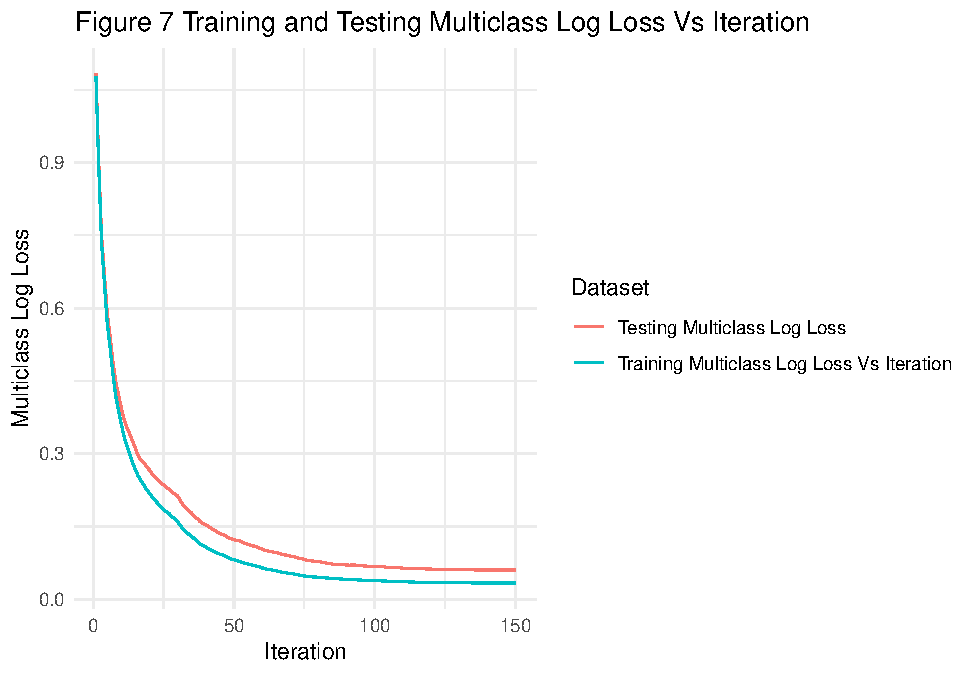
\includegraphics{Code_C_files/figure-latex/plot of multicalss log loss graph-1.pdf}
Figure 7 illustrates the Multiclass Log Loss for both the training and
testing datasets across iterations during model training. Initially,
both the training and testing log-loss values are extremely high,
indicating poor predictions.

As the training process (iteration grows up), log-loss decreases
sharply, showing that the model's performance is getting better. The
training log-loss stays below the testing log-loss is normal, because
the model perform better on training data obviously.

Moreover, when iteration grows to over 75, the model is approaching its
optimal performance, because both training and testing curves converge.
Meanwhile, the gap between Training and Testing multiclass log loss
remain small, and this demonstrates good generalization to the testing
data.

In conclusion, by applying grid search, I fit a new model that achieves
higher Test Weighted F1-Score than the original model, which means the
new model can perform better when classifying unseen data.

\subsection*{Reference}\label{reference}
\addcontentsline{toc}{subsection}{Reference}

\phantomsection\label{refs}
\begin{CSLReferences}{1}{0}
\bibitem[\citeproctext]{ref-10.1214ux2f09-SS054}
Arlot, Sylvain, and Alain Celisse. 2010. {``A Survey of Cross-Validation
Procedures for Model Selection.''} \emph{Statistics Surveys} 4: 40--79.
\url{https://doi.org/10.1214/09-SS054}.

\bibitem[\citeproctext]{ref-NIPS2011_86e8f7ab}
Bergstra, James, Rémi Bardenet, Yoshua Bengio, and Balázs Kégl. 2011.
{``Algorithms for Hyper-Parameter Optimization.''} In \emph{Advances in
Neural Information Processing Systems}, edited by J. Shawe-Taylor, R.
Zemel, P. Bartlett, F. Pereira, and K. Q. Weinberger. Vol. 24.
\url{https://proceedings.neurips.cc/paper_files/paper/2011/file/86e8f7ab32cfd12577bc2619bc635690-Paper.pdf}.

\bibitem[\citeproctext]{ref-car_evaluation_19}
Bohanec, Marko. 1988. {``Car Evaluation.''} UCI Machine Learning
Repository.

\bibitem[\citeproctext]{ref-chen2016xgboost}
Chen, Tianqi, and Carlos Guestrin. 2016. {``XGBoost: A Scalable Tree
Boosting System.''} In \emph{Proceedings of the 22nd ACM SIGKDD
International Conference on Knowledge Discovery and Data Mining},
785--94. ACM.

\bibitem[\citeproctext]{ref-app14219863}
Hinojosa Lee, Maria Cristina, Johan Braet, and Johan Springael. 2024.
{``Performance Metrics for Multilabel Emotion Classification: Comparing
Micro, Macro, and Weighted F1-Scores.''} \emph{Applied Sciences} 14
(21). \url{https://doi.org/10.3390/app14219863}.

\end{CSLReferences}

\end{document}
